\section{Kiểm chứng và đánh giá thực nghiệm}
\label{sec:experiments}

\subsection{Chiến lược kiểm chứng}

Việc đánh giá dự án dựa trên kết quả kiểm thử và số liệu đo được. Một bước chỉ được ghi \ident{PASS} khi có bằng chứng xác nhận; bước chưa chạy được ghi \ident{NOT_RUN} kèm lý do. Tương tự, bộ công cụ benchmark giữ giá trị \ident{null} cho chỉ số chưa đo được và ghi rõ nguyên nhân. Các mục tiêu thiết kế, chẳng hạn p95 $<$ 10 s, được trình bày riêng để người đọc có thể đối chiếu với kết quả thực tế.

\subsubsection{Các tầng kiểm thử}

Bảng~\ref{tab:testlayers} trình bày phạm vi và hạ tầng của từng tầng kiểm thử. Số hàm kiểm thử trong bảng được đếm trực tiếp từ mã nguồn. Khi chạy, số trường hợp kiểm thử lớn hơn số hàm vì một hàm có thể được chạy với nhiều bộ tham số thông qua \ident{pytest.mark.parametrize}.

\begin{table}[H]
\centering
\tablefont
\caption{Các tầng kiểm thử}
\label{tab:testlayers}
\begin{tabular}{p{2.21cm}p{1.19cm}p{1.38cm}p{5.90cm}p{3.32cm}}
\toprule
\textbf{Tầng} & \textbf{Số tệp} & \textbf{Hàm test} & \textbf{Phạm vi} & \textbf{Hạ tầng} \\
\midrule
Unit & 38 & 438 & ID, quy tắc xử lý, lịch GTFS/DST, lịch dịch vụ, phạm vi, outbox, HTTP giả lập, API với repository giả, replay, oracle & Python thuần \\
Runtime & 18 & 133 & Checksum, giải nén an toàn, supervisor/registry, phiên chạy, reset, doctor, tunnel, xuất dữ liệu & Python thuần \\
Spark & 12 & 117 & Phân tích dữ liệu, vị trí xe, dự báo, KPI, cảnh báo, ghi và công bố dữ liệu, curated, truy vết trên golden fixture & JDK + PySpark \texttt{local[1]} \\
Integration & 10 & 18 & IT01--IT16 với Kafka, Cassandra, Spark thực tế qua native runner & Toàn hệ thống \\
Golden smoke & -- & 5 bước & Golden fixture qua Kafka $\rightarrow$ Spark $\rightarrow$ Cassandra $\rightarrow$ API & Toàn hệ thống \\
\bottomrule
\end{tabular}
\end{table}

\subsubsection{Golden fixture và oracle độc lập}

Golden fixture tại \ident{tests/fixtures/golden/} là bộ dữ liệu kiểm thử \textbf{được tạo thủ công, không phải dữ liệu MBTA}. Bộ dữ liệu này gồm GTFS tĩnh với đơn vị vận hành \ident{SYN}, hai tuyến \ident{R_A}, \ident{R_B}, các trạm từ \ident{S1} đến \ident{S9} và ba feed VP/TU/Alerts có cấu trúc tương tự JSON của MBTA. Các giá trị kỳ vọng trong \ident{expected.json} đều được tính bằng tay từ đặc tả thiết kế, mỗi giá trị được tính độc lập hai lần. Nhờ đó, kết quả kỳ vọng không phụ thuộc vào kết quả do hệ thống tạo ra. Bảng thời gian epoch trong \ident{PROVENANCE.md} cũng được kiểm tra bằng test.

Dự án còn dùng một \textbf{oracle độc lập} tại \ident{tests/oracle/} để tính lại kết quả bằng thư viện chuẩn Python. Test \ident{test_oracle_isolation.py} phân tích cây cú pháp AST và chạy tiến trình con để kiểm tra rằng oracle không import \ident{transitpulse} hoặc \ident{pyspark}. Chuỗi đối chiếu gồm oracle(fixture) $=$ \ident{expected.json} và pipeline (Spark, API, Cassandra) $=$ \ident{expected.json}. Cách kiểm chứng qua ba nguồn độc lập giúp giảm khả năng phần xử lý và kết quả kỳ vọng cùng mắc một lỗi.

\subsubsection{Kịch bản golden}

Kịch bản golden gồm năm bước. Sau mỗi bước, bộ phát dữ liệu (publisher) và bộ xử lý (processor) chờ nhau tại một điểm đồng bộ (barrier) trước khi tiếp tục. Bảng~\ref{tab:golden} trình bày các giá trị kỳ vọng chính của tuyến \ident{R_A}.

\begin{longtable}{p{1.06cm}p{3.85cm}p{10.22cm}}
\caption{Năm bước của kịch bản golden và giá trị kỳ vọng chính (tuyến R\_A)} \label{tab:golden} \\
\toprule
\textbf{Bước} & \textbf{Đầu vào (đồng hồ)} & \textbf{Kỳ vọng} \\
\midrule
\endfirsthead
\toprule
\textbf{Bước} & \textbf{Đầu vào (đồng hồ)} & \textbf{Kỳ vọng} \\
\midrule
\endhead
{\tablefont S1} & {\tablefont VP1, TU1, ALERTS1 (12:00:30Z)} & {\tablefont Ba con trỏ được tạo. Xe: fresh 1, stale 1, unknown 1, membership 3. KPI: 2 trip instance, eligible 2, late 1, rate 0,5, mean 210 s. Tuyến R\_B không có chuyến: rate và mean là \texttt{null}.} \\
{\tablefont S2} & {\tablefont VP2 (12:01:00Z)} & {\tablefont Con trỏ VP chuyển sang VP2. Xe V2 vắng trong VP2 nên không còn được tính: fresh 1, unknown 1, membership 2. Lịch sử V1 và V3 mỗi xe có 2 dòng.} \\
{\tablefont S3} & {\tablefont Phát lại VP2 (12:01:00Z)} & {\tablefont VP2 được phát lại khi đang là snapshot hiện hành: không tạo generation mới, con trỏ giữ nguyên, lịch sử không tăng, bộ đếm duplicate VP $=$ 1.} \\
{\tablefont S4} & {\tablefont Phát lại VP1 (12:01:00Z)} & {\tablefont VP1 vừa trùng vừa đến muộn: con trỏ \textbf{không lùi} về VP1, lịch sử không đổi, duplicate VP $=$ 2, late VP $=$ 1, có bản ghi audit \texttt{LATE\_SNAPSHOT\_NOT\_PUBLISHED}.} \\
{\tablefont S5} & {\tablefont Chỉ tiến đồng hồ (12:03:10Z)} & {\tablefont Không có dữ liệu mới nhưng trạng thái thay đổi theo đồng hồ: feed VP tuổi 130 s (stale), TU tuổi 170 s (stale, ngưỡng 90 s), Alerts tuổi 170 s (chưa stale, ngưỡng 300 s). Xe: fresh 0, stale 1, unknown 1. KPI giữ giá trị của generation nhưng được đánh dấu stale.} \\
\bottomrule
\end{longtable}

\subsubsection{Kịch bản tích hợp}

Bảng~\ref{tab:it} liệt kê 16 kịch bản kiểm thử tích hợp với Kafka, Cassandra và Spark thực tế. Hai kịch bản gây gián đoạn môi trường, gồm IT12 dừng Cassandra và IT16 tắt mạng, được bố trí chạy cuối.

\begin{table}[H]
\centering
\tablefont
\caption{Kịch bản tích hợp IT01--IT16}
\label{tab:it}
\begin{tabular}{p{1.07cm}p{5.27cm}p{8.79cm}}
\toprule
\textbf{Mã} & \textbf{Kịch bản} & \textbf{Điều kiện đạt} \\
\midrule
IT01 & Golden fixture ban đầu & Số đếm, tỉ lệ 0,5 và trung bình 210 s khớp tại API và nơi ghi dữ liệu \\
IT02 & Snapshot mới phát hai lần & Membership không tăng; lịch sử không lặp cùng quan sát \\
IT03 & Snapshot cũ tới sau snapshot mới & Con trỏ và vị trí không lùi; snapshot đến muộn có audit \\
IT04 & Đồng hồ tiến, không có vị trí mới & Xe chuyển stale; dự báo cũ báo stale \\
IT05 & Snapshot rỗng hợp lệ và dữ liệu sai định dạng/timeout & Lỗi nguồn không biến thành snapshot rỗng \\
IT06 & Thiếu timestamp, GPS không hợp lệ & Unknown không được tính là fresh; cách xử lý và số đếm đúng \\
IT07 & Ngày dịch vụ không rõ, trạm lặp & Không tự đoán lịch hoặc trạm; ghi lý do khi loại khỏi KPI \\
IT08 & Uncertainty bus, chuyến bị hủy & Các giá trị 300, 301, $>$301 và trường hợp thiếu được xử lý đúng quy tắc \\
IT09 & Cảnh báo cập nhật một phần & Không đóng hàng loạt cảnh báo cũ; thông tin truy vết được kế thừa đúng \\
IT10 & Dừng sau khi ghi một phần & API giữ generation cũ; khởi động lại hoàn tất đúng generation \\
IT11 & Dừng sau CAS, trước commit checkpoint & Dùng lại generation READY; thời điểm công bố đầu tiên và TTL không đổi \\
IT12 & Cassandra dừng & Batch thất bại; offset không được coi là đã xử lý \\
IT13 & Message gần 4 MiB và vượt ngưỡng & Kiểm tra đúng giới hạn kích thước; thông điệp vượt ngưỡng vào DLQ \\
IT14 & Cô lập run, tạm dừng replay & Kết quả tách theo run; đồng hồ nghiệp vụ dừng, heartbeat theo giờ máy tiếp tục \\
IT15 & Generation hết TTL & 503 \texttt{generation\_expired}, phân biệt với 0 dòng hợp lệ \\
IT16 & Demo khi tắt mạng & Pipeline, API và giao diện lõi vẫn dùng được \\
\bottomrule
\end{tabular}
\end{table}

Mỗi lần push hoặc tạo pull request, CI trên GitHub Actions chạy Ruff, các kiểm thử unit và runtime, đồng thời kiểm tra tĩnh notebook, cấu hình, fixture và migration. Các kiểm thử tích hợp được chạy qua một workflow kích hoạt thủ công.

\subsection{Môi trường thực nghiệm}

Số liệu thực nghiệm được lấy từ hai lần chạy trên Google Colab với cùng một loại máy ảo. Cấu hình môi trường được trình bày trong Bảng~\ref{tab:env}. Hai lần chạy gồm:
\begin{itemize}
    \item \textbf{Demo (Run All)} ngày 19/10/2026, tại commit \ident{4d6669e}: dựng môi trường, chạy kiểm thử, golden smoke, thu thập trực tiếp trên 10 tuyến và truy vết dữ liệu. Số liệu được lấy từ kết quả đã lưu trong notebook \ident{TransitPulse_MBTA_Colab_Demo.ipynb} và ảnh chụp giao diện React của phiên chạy này.
    \item \textbf{Benchmark} ngày 24/10/2026, tại commit \ident{ff49f59}: chạy ba kịch bản tải cao và bốn kịch bản phục hồi. Số liệu được lấy từ thư mục kết quả \ident{bench-20261024T182433Z} do bộ công cụ benchmark tạo ra.
\end{itemize}
Các thay đổi giữa hai lần chạy gồm bổ sung cache \ident{persist} cho kết quả của builder, ghi log thời gian theo từng giai đoạn và bổ sung phần benchmark. Các thay đổi này giữ nguyên ngữ nghĩa xử lý dữ liệu.

\begin{table}[H]
\centering
\tablefont
\caption{Môi trường chạy thực nghiệm (Google Colab, profile colab-native)}
\label{tab:env}
\begin{tabular}{p{4.20cm}p{11.40cm}}
\toprule
\textbf{Hạng mục} & \textbf{Giá trị quan sát} \\
\midrule
Hệ điều hành / kiến trúc & Linux, x86\_64, chạy với quyền root (Cassandra khởi động với cờ \texttt{-R}) \\
CPU & 8 CPU logic (AMD EPYC 7B12) \\
RAM & 54\,750\,396\,416 B ($\approx$ 51,0 GiB); khả dụng lúc kiểm tra $\approx$ 49,4 GiB \\
Đĩa trống & 216\,798\,367\,744 B ($\approx$ 201,9 GiB) \\
Phần mềm & Python 3.11.17, Temurin 17.0.20.1+1, Kafka 4.2.2, Cassandra 5.0.9, PySpark 3.5.7, Node.js 22.21.0, cloudflared 2026.10.0 \\
Cấu hình & Spark \texttt{local[2]}, driver 16 GiB, whole-stage codegen tắt; Kafka heap 1 GiB; Cassandra heap 4 GiB + direct 2 GiB \\
Phạm vi live & 10 tuyến xe buýt; \texttt{gtfs\_version} \texttt{8dc7ee14\ldots6c6205}; \texttt{scope\_id} \texttt{de5bf686d21385a5}; múi giờ \texttt{America/New\_York} \\
\bottomrule
\end{tabular}
\end{table}

\subsection{Kết quả}

\subsubsection{Bootstrap và hạ tầng}

Bảng~\ref{tab:bootstrap} tổng hợp thời gian dựng môi trường. Trong bước bootstrap, hệ thống tải năm gói phần mềm và đối chiếu checksum với thông tin chính thức: JDK dùng SHA-256 từ Adoptium API, Kafka dùng SHA-512, Cassandra và Node.js dùng SHA-256, còn cloudflared dùng SHA-256 trong release notes. Cả năm gói đều có checksum trùng khớp. Tệp \ident{uv.lock} được tạo trên Colab với \ident{lock_origin=generated_on_colab}, sau khi công cụ xác định phiên bản cho 69 gói phụ thuộc. Công cụ Doctor ghi nhận PASS ở mọi kiểm tra và một WARN do \ident{uv.lock} chưa được commit vào repository.

\begin{table}[H]
\centering
\tablefont
\caption{Thời gian dựng môi trường trên Colab}
\label{tab:bootstrap}
\begin{tabular}{p{5.43cm}p{2.13cm}p{7.57cm}}
\toprule
\textbf{Bước} & \textbf{Thời gian} & \textbf{Kết quả} \\
\midrule
Bootstrap (uv, Python, JDK, Kafka, Cassandra, Node, biên dịch React, connector) & 104,8 s & PASS, chạy lần đầu, chưa có cache \\
Doctor / preflight & 0,6 s & PASS (1 WARN: \texttt{lock\_origin}) \\
Kafka KRaft sẵn sàng & 3,7 s & READY, khởi tạo cluster mới \\
Cassandra sẵn sàng & 42,6 s & READY, phiên bản 5.0.9 \\
Khởi tạo hạ tầng (topic + CQL migration) & 9,8 s & 5 topic CREATED, migration \texttt{0001\_initial} APPLIED, TTL probe PASS \\
\bottomrule
\end{tabular}
\end{table}

\subsubsection{Kiểm thử unit, runtime và Spark}

Lệnh \ident{pytest -m 'unit or runtime or spark'} hoàn tất với \textbf{940 passed, 1 warning} sau 995,68 s, tương đương 16 phút 35 giây. Cảnh báo duy nhất là \ident{StarletteDeprecationWarning} từ \ident{fastapi.testclient}, không liên quan đến logic của dự án. Các kiểm thử Spark chiếm phần lớn thời gian do mỗi test phải khởi tạo và giải phóng cache trên Spark session \ident{local[1]}. Kết quả này kiểm chứng các phép biến đổi ở mức unit; việc phối hợp giữa các thành phần vẫn cần được đánh giá bằng kiểm thử tích hợp.

\subsubsection{Golden smoke end-to-end}

Golden smoke đưa bộ dữ liệu golden qua toàn bộ hệ thống: publisher $\rightarrow$ Kafka $\rightarrow$ Spark $\rightarrow$ Cassandra $\rightarrow$ API. Sau mỗi bước, kết quả đọc từ API được đối chiếu với \ident{expected.json}. Cả năm bước đều \textbf{PASS}, không có kiểm tra nào thất bại. Thời gian và kết quả từng bước được trình bày trong Bảng~\ref{tab:goldenrun}.

\begin{table}[H]
\centering
\tablefont
\caption{Kết quả golden smoke (run \texttt{5cece312\ldots}, tổng 266,2 s)}
\label{tab:goldenrun}
\begin{tabular}{p{6.21cm}p{2.32cm}p{6.60cm}}
\toprule
\textbf{Giai đoạn} & \textbf{Thời gian} & \textbf{Kết quả} \\
\midrule
Sinh fixture (\texttt{synth-generate golden}) & 0,4 s & exit 0 \\
Nạp dữ liệu tĩnh (Spark batch + Cassandra) & 42,5 s & exit 0, phạm vi dữ liệu tĩnh đã được công bố \\
Bộ xử lý / API / bộ phát sẵn sàng & 10,0 / 2,2 / 1,0 s & READY \\
Bước S1 (ba feed đầu tiên) & 165 s & PASS \\
Bước S2 (VP mới) & 25 s & PASS \\
Bước S3 (phát lại dữ liệu trùng) & 7 s & PASS \\
Bước S4 (dữ liệu trùng, đến muộn) & 4 s & PASS \\
Bước S5 (chỉ tiến đồng hồ) & 5 s & PASS \\
\bottomrule
\end{tabular}
\end{table}

Thời gian trong bảng được tính từ lúc publisher đến điểm đồng bộ cho tới khi toàn bộ kiểm tra của bước đó PASS. Vì vậy, số liệu này phản ánh thời gian hoàn tất bước kiểm thử, khác với độ trễ từ lúc phát dữ liệu đến lúc dữ liệu có thể được đọc qua API (visibility latency). Bước S1 mất 165 s do bao gồm các micro-batch đầu tiên sau khi JVM khởi động. Spark phải lập kế hoạch và thực thi lần đầu cho cả ba feed, trong đó nhánh dự báo có kế hoạch xử lý phức tạp nhất. Các bước còn lại mất 4--25 s; S3 và S4 nhanh nhất vì dữ liệu trùng hoặc đến muộn không tạo generation mới. Qua toàn bộ pipeline, kết quả xác nhận các yêu cầu chính của FR05, FR07 và FR10: số xe không cộng dồn giữa các snapshot, mỗi chuyến chỉ có một target để tính KPI, bản ghi trùng không làm tăng lịch sử, con trỏ không lùi khi snapshot đến muộn và độ mới được cập nhật theo đồng hồ dù không có dữ liệu mới.

\subsubsection{Thu thập trực tiếp dữ liệu MBTA}

Sau golden smoke, notebook tiếp tục chạy một phiên thu thập trực tiếp trong 600 giây trên 10 tuyến xe buýt. Bảng~\ref{tab:live} tóm tắt các giai đoạn của phiên chạy.

\begin{table}[H]
\centering
\tablefont
\caption{Các giai đoạn phiên thu thập trực tiếp (run \texttt{1908043e\ldots})}
\label{tab:live}
\begin{tabular}{p{6.40cm}p{2.32cm}p{6.40cm}}
\toprule
\textbf{Giai đoạn} & \textbf{Thời gian} & \textbf{Ghi chú} \\
\midrule
Tải GTFS ZIP của MBTA & $\approx$ 1 s & \texttt{static\_download ok} \\
Spark trích xuất và kiểm tra & $\approx$ 87 s & Kiểm tra dữ liệu tĩnh PASSED; 10/10 tuyến hợp lệ, không có tuyến bị loại \\
Ghi các bảng chiều dạng Parquet & $\approx$ 13 s & \texttt{static\_write\_parquet ok} \\
Ghi danh mục dữ liệu tĩnh vào Cassandra & $\approx$ 260 s & riêng \texttt{stop\_times\_by\_trip} $\approx$ 253 s \\
\textbf{Tổng thời gian nạp dữ liệu tĩnh} & \textbf{367,6 s} & \\
Khởi động bộ xử lý / bộ thu thập & 11,0 / 1,0 s & Dùng lại tiến trình API của golden smoke \\
Chờ generation READY đầu tiên & 38,6 s & VP READY; \texttt{/health/ready}, \texttt{/runs}, \texttt{/quality} trả 200 \\
\bottomrule
\end{tabular}
\end{table}

Việc nạp GTFS thực tế của MBTA mất thời gian gần gấp 9 lần so với bộ fixture. Khoảng 70\% thời gian nạp dành cho việc ghi bảng \ident{stop_times_by_trip} vào Cassandra, cho thấy đây là bước chậm nhất của quá trình nạp dữ liệu tĩnh trong lần chạy này. Hướng cải thiện được trình bày ở Phần~\ref{sec:conclusion}.

\subsubsection{Truy vết dữ liệu và độ trễ công bố}

Lệnh \ident{demo.py lineage} được chạy lúc 13:47:23Z để truy vết generation VP hiện hành. Kết quả \textbf{PASS}, với thông tin nhất quán giữa các tầng từ dữ liệu gốc đến API như trình bày trong Bảng~\ref{tab:lineage}.

\begin{table}[H]
\centering
\tablefont
\caption{Truy vết snapshot \texttt{sn\_33e812db\ldots} (feed vehicle\_positions)}
\label{tab:lineage}
\begin{tabular}{p{2.20cm}p{13.40cm}}
\toprule
\textbf{Tầng} & \textbf{Quan sát} \\
\midrule
Con trỏ & \texttt{is\_current = true}; \texttt{generation\_id gn\_1689bd0c\ldots}; \texttt{view\_published\_at} 13:47:11.842Z; \texttt{expires\_at} 14:46:46.679Z \\
Manifest & \texttt{READY}, \texttt{publish\_outcome = PUBLISHED}; \texttt{published\_at} 13:46:37.017Z; \texttt{ready\_at} 13:47:11.829Z; \texttt{visibility\_latency\_ms} = 34\,825 \\
Raw & Nội dung JSON 310\,371 B, nén gzip còn 33\,767 B; SHA-256 kỳ vọng và thực tế trùng khớp (\texttt{465ca68e\ldots}) \\
Kafka & Topic \texttt{mbta.vehicle\_positions.snapshots.v1}, partition 0, offset 5; envelope 40\,512 B; \texttt{snapshot\_id} và \texttt{capture\_id} trong header khớp envelope \\
Batch & \texttt{first\_batch\_id} = 2 \\
API & HTTP 200 trên \texttt{/vehicles}, trả đúng \texttt{snapshot\_id} của con trỏ \\
\bottomrule
\end{tabular}
\end{table}

Kết quả truy vết cho thấy các điểm sau:
\begin{itemize}
    \item \textbf{Lưu trữ và lọc theo phạm vi.} Nội dung Vehicle Positions của toàn mạng MBTA có kích thước 310\,371 B. Sau khi nén gzip, kích thước giảm khoảng 9,2 lần. Khi chỉ giữ dữ liệu của 10 tuyến, thông điệp envelope trên Kafka còn 40\,512 B, tương đương khoảng 13\% nội dung gốc.
    \item \textbf{Thời gian ở từng bước xử lý.} Visibility latency của mẫu này là 34,8 s. Theo các mốc trong manifest, từ lúc generation đạt READY đến khi con trỏ được cập nhật bằng CAS chỉ mất 13 ms. Như vậy, gần như toàn bộ độ trễ phát sinh trước READY. Ở chế độ live, \ident{metrics_as_of} được cố định trong manifest theo giờ máy lúc bộ xử lý bắt đầu xử lý snapshot, ở đây là 13:46:46.679Z. Dựa vào mốc này, có thể ước lượng khoảng 9,7 s từ lúc phát dữ liệu đến lúc bộ xử lý bắt đầu xử lý, bao gồm thời gian chờ trigger, chờ micro-batch trước và phân tích dữ liệu. Khoảng 25,2 s còn lại dành cho xây dựng generation, ghi Cassandra và công bố kết quả. Với generation VP đầu tiên của phiên chạy, khoảng thời gian từ lúc bắt đầu xây dựng đến lúc có thể đọc được là 34,7 s.
    \item \textbf{Đối chiếu với mục tiêu.} Độ trễ của mẫu đơn lẻ này \textbf{lớn hơn ngưỡng của mục tiêu p95 $<$ 10 s}. Tại thời điểm truy vết, TU và Alerts chưa có generation READY, đồng thời dữ liệu curated của batch 2 chưa được commit. Điều này cho thấy micro-batch vẫn xử lý các feed còn lại sau khi VP đã được công bố. Mục~\ref{sec:ui} trình bày độ trễ lớn hơn của TU và Alerts trong cùng micro-batch; nguyên nhân được phân tích ở Mục~\ref{sec:bench}.
    \item \textbf{Độ mới của nguồn.} Tại thời điểm truy vết, feed VP có tuổi 49,2 s, vẫn dưới ngưỡng stale 120 s.
\end{itemize}

\subsubsection{Giao diện trong phiên thu thập trực tiếp}
\label{sec:ui}

Hình~\ref{fig:ui-map}, \ref{fig:ui-stops} và \ref{fig:ui-overview} ghi lại giao diện React trong phiên thu thập trực tiếp, với run \texttt{1908043e\ldots} và tuyến 1 Harvard Square -- Nubian Station. Các ảnh được chụp trong khoảng 13:55--13:56 UTC, gần cuối phiên chạy 600 s.

\begin{figure}[H]
\centering
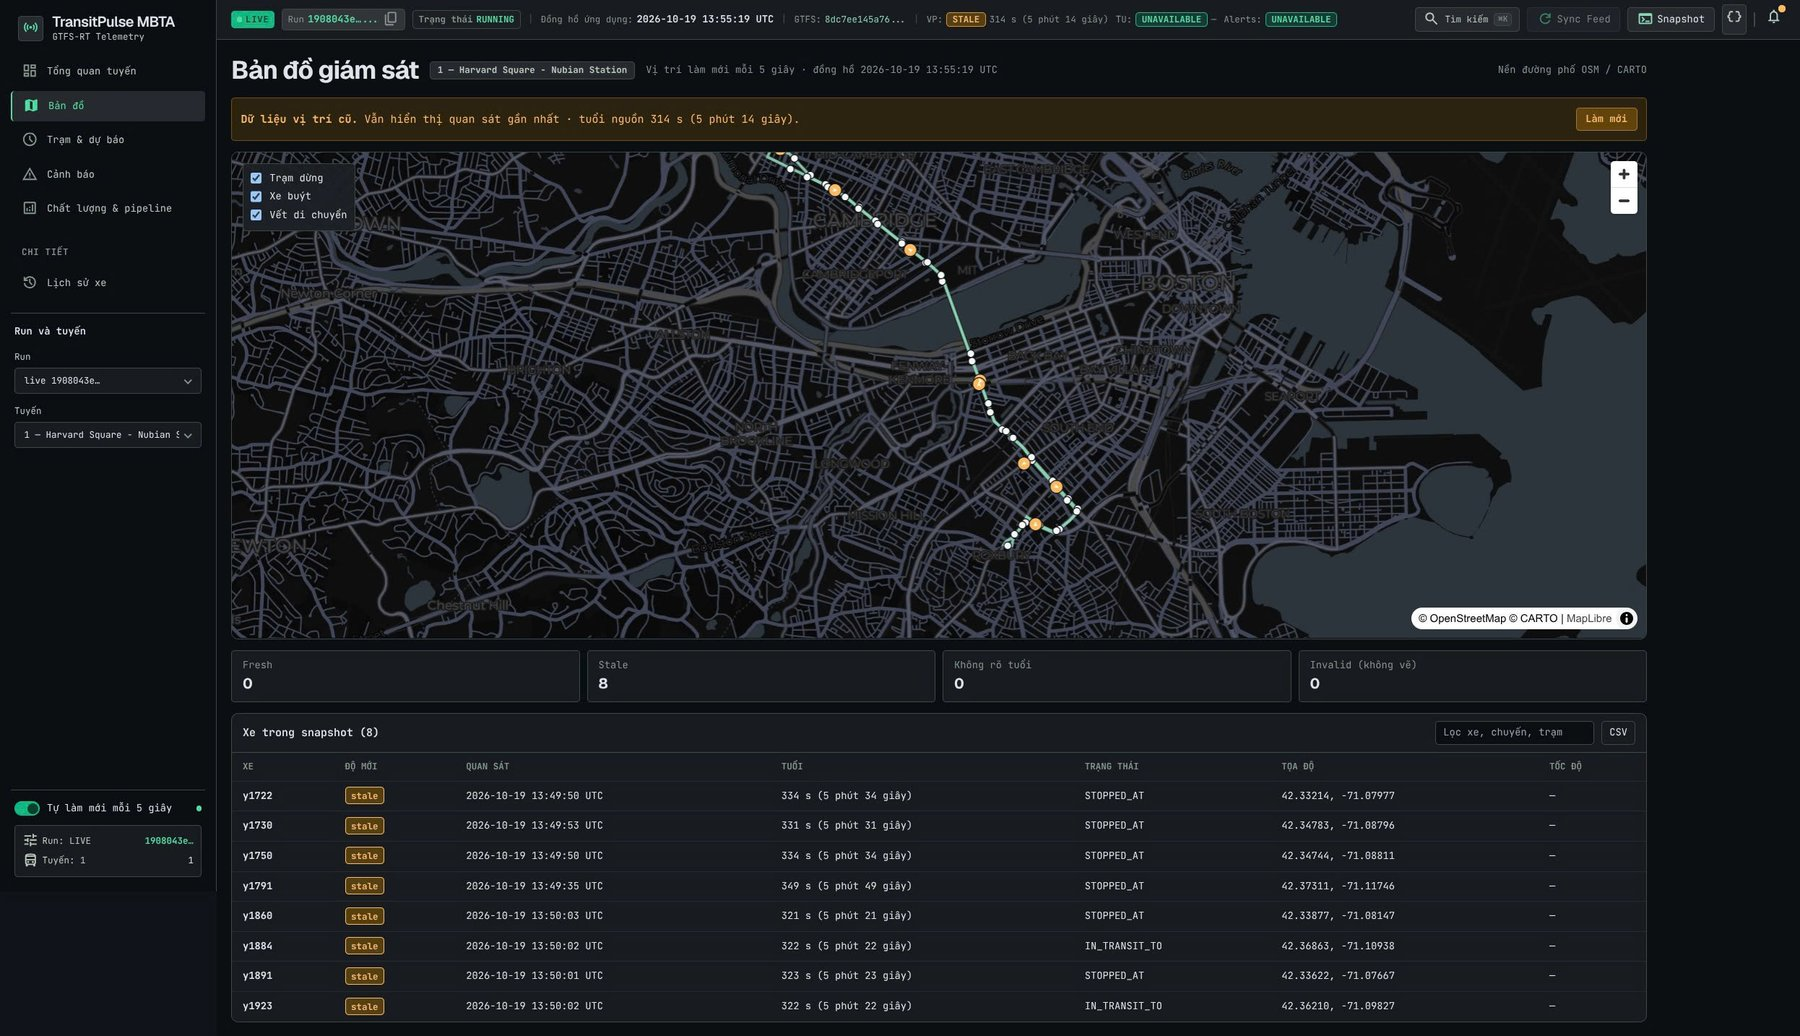
\includegraphics[width=\textwidth]{ui_map.jpg}
\caption{Màn hình Bản đồ hiển thị 8 xe tuyến 1 trên nền CARTO/OpenStreetMap. Cả 8 xe đều ở trạng thái stale, với tuổi dữ liệu 321--349 s so với ngưỡng 120 s. Giao diện giữ vị trí xe và hiển thị thông báo ``Dữ liệu vị trí cũ''.}
\label{fig:ui-map}
\end{figure}

\begin{figure}[H]
\centering
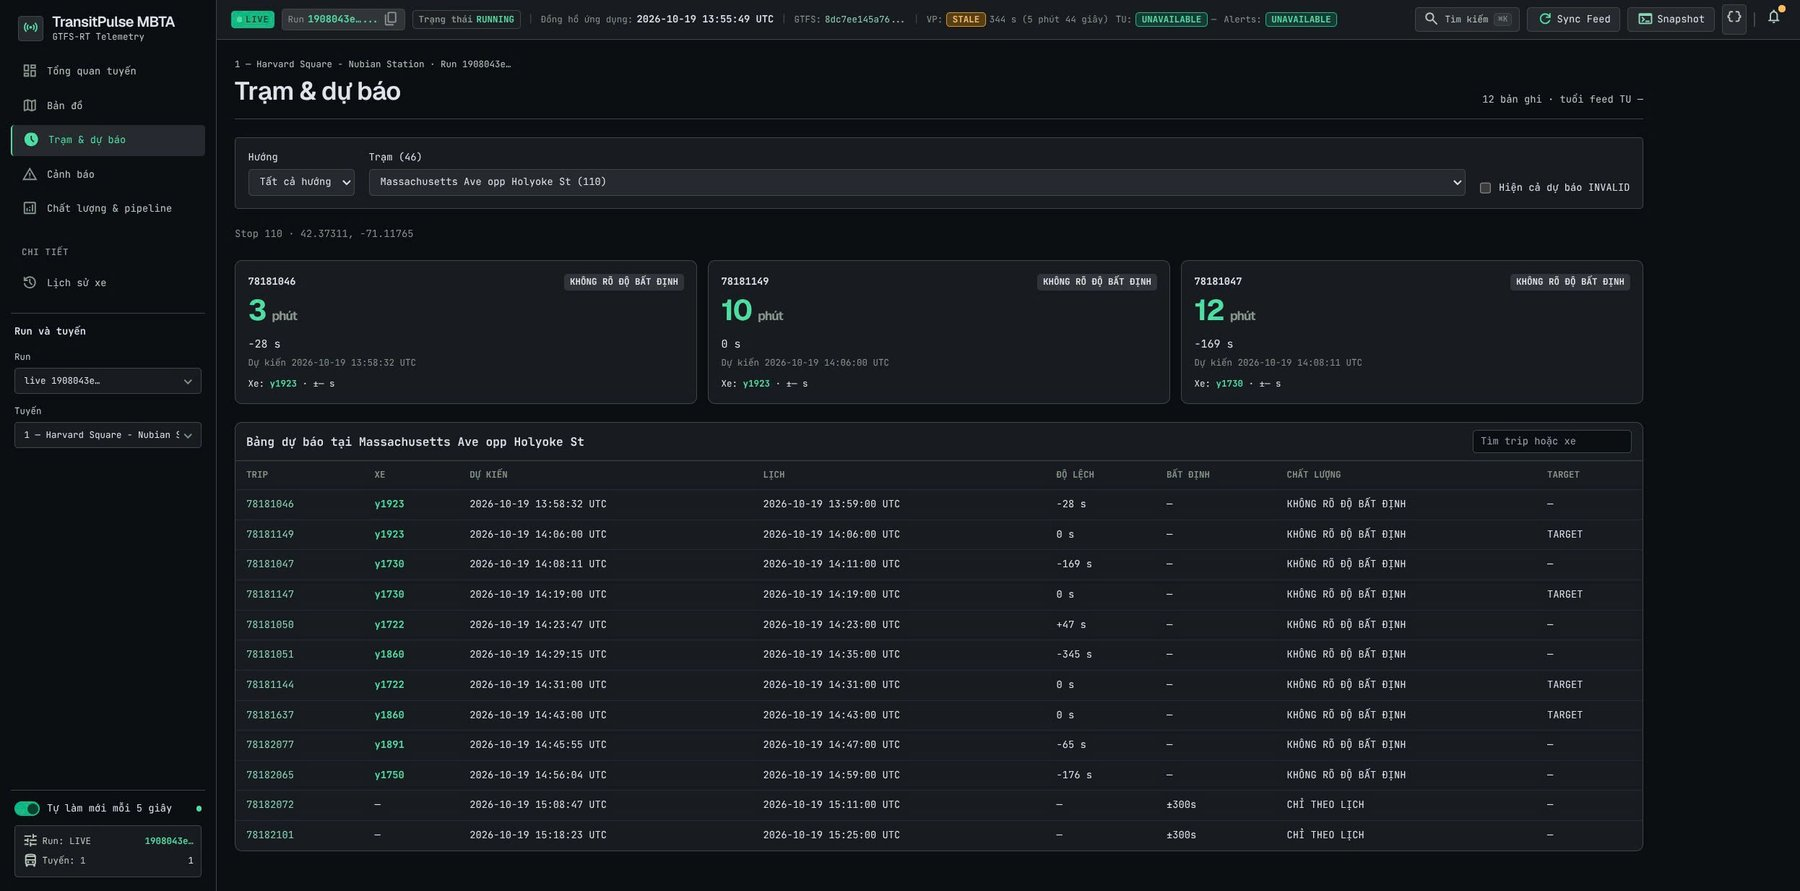
\includegraphics[width=\textwidth]{ui_stops.jpg}
\caption{Màn hình Trạm \& dự báo tại trạm 110 (Massachusetts Ave opp Holyoke St) hiển thị giờ dự kiến, giờ theo lịch, độ lệch có thể âm, nhãn chất lượng và cờ TARGET của từng chuyến. Hai dòng cuối là dự báo chỉ dựa trên lịch, với uncertainty bằng 300.}
\label{fig:ui-stops}
\end{figure}

\begin{figure}[H]
\centering
\begin{subfigure}{\textwidth}
\centering
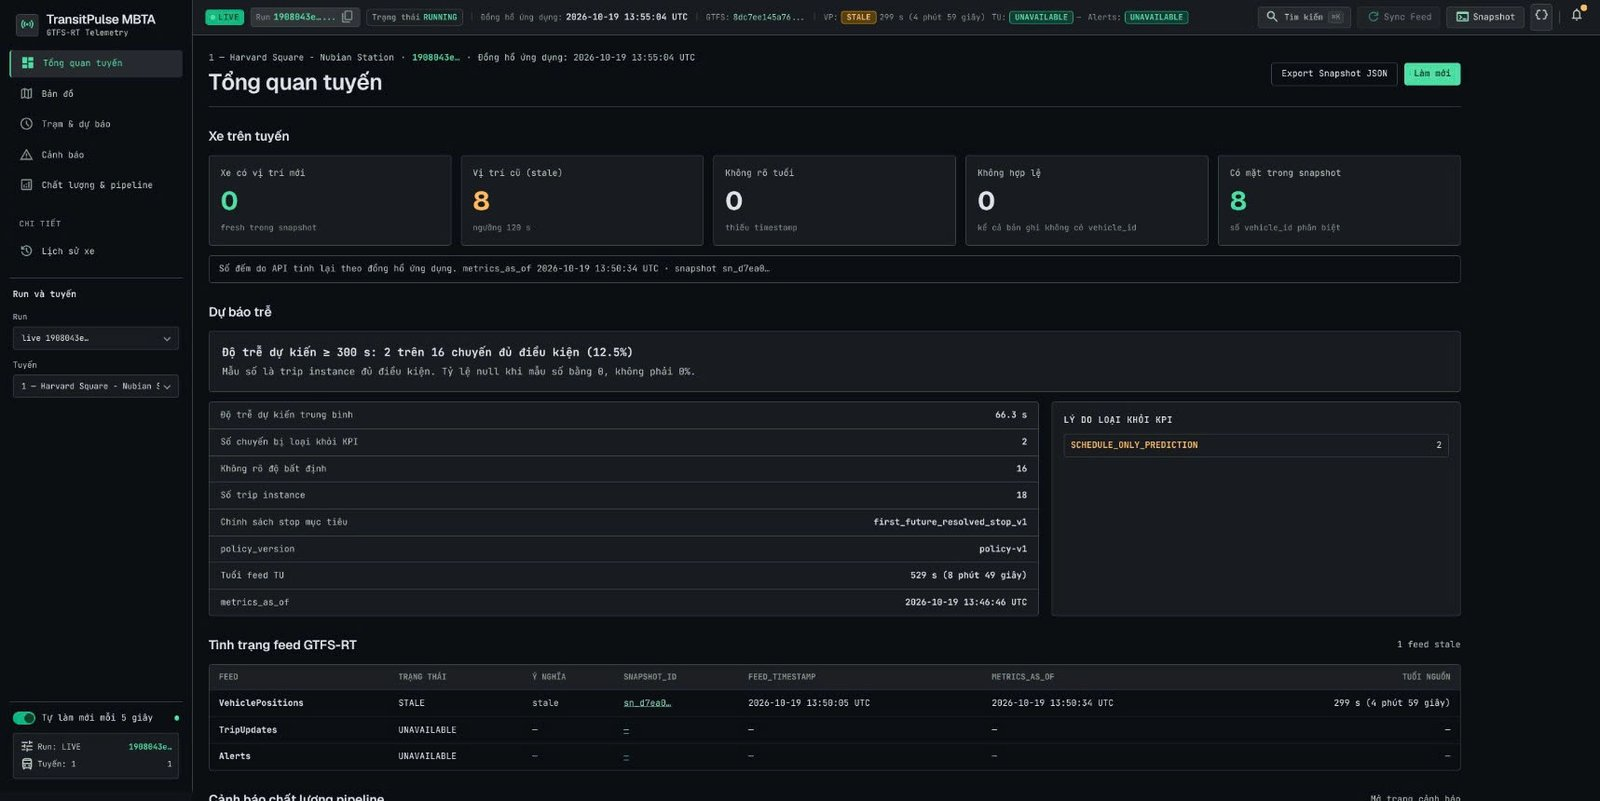
\includegraphics[width=\textwidth]{ui_overview.jpg}
\caption{Màn hình Tổng quan tuyến hiển thị số xe theo mức độ mới, KPI độ trễ dự kiến kèm mẫu số và lý do loại trừ, cùng trạng thái của từng feed.}
\end{subfigure}

\vspace{4mm}
\begin{subfigure}{\textwidth}
\centering
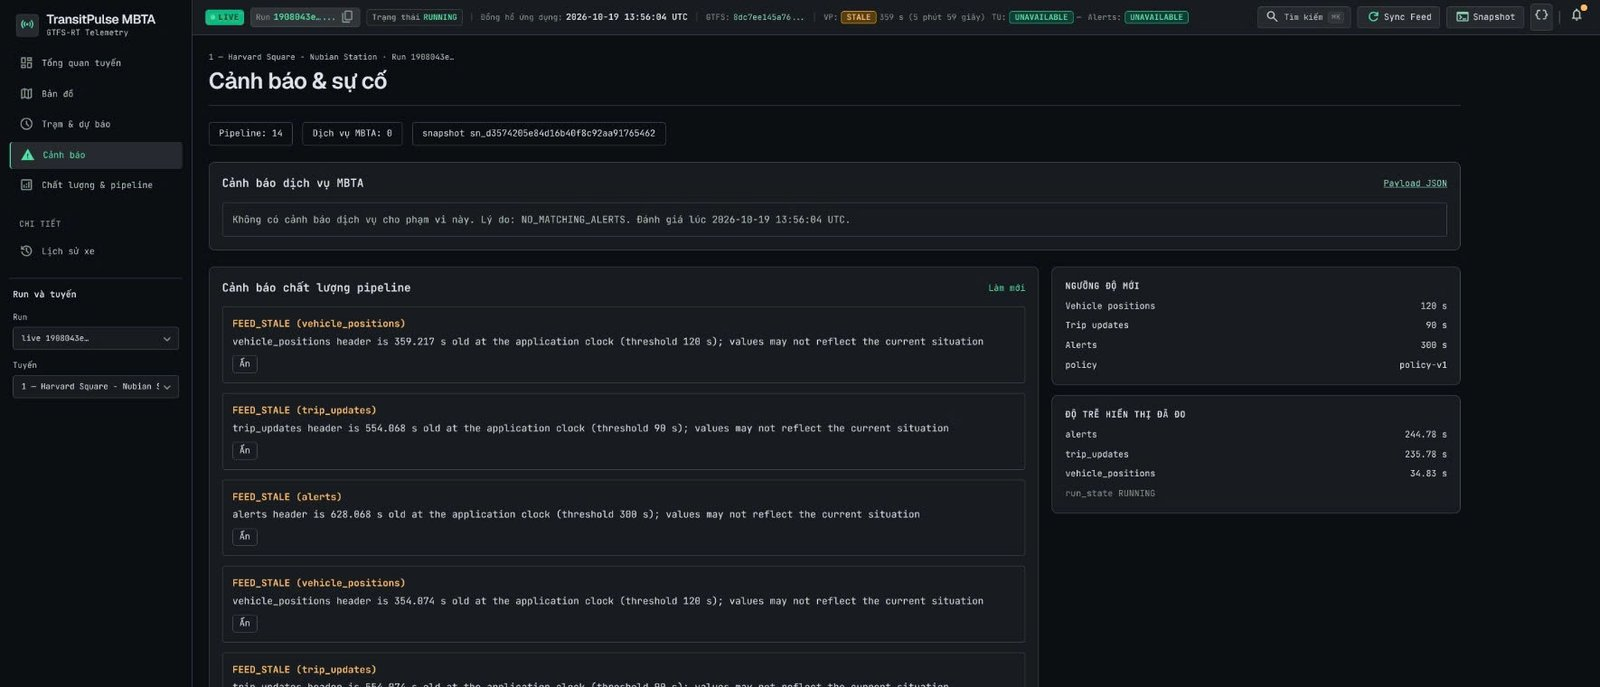
\includegraphics[width=\textwidth]{ui_alerts.jpg}
\caption{Màn hình Cảnh báo trình bày riêng cảnh báo dịch vụ MBTA và cảnh báo chất lượng pipeline. Khung bên phải hiển thị visibility latency gần nhất của từng feed.}
\end{subfigure}
\caption{Màn hình Tổng quan và Cảnh báo trên giao diện React; ảnh đã cắt phần dưới.}
\label{fig:ui-overview}
\end{figure}

Từ các ảnh chụp, có thể ghi nhận thêm bốn điểm trên dữ liệu thực tế:
\begin{itemize}
    \item \textbf{Số lượng chuyến dùng để tính KPI khớp.} Tuyến 1 có 18 trip instance, trong đó 16 chuyến đủ điều kiện và 2 chuyến bị loại với lý do \texttt{SCHEDULE\_ONLY\_PREDICTION}. Các số đếm thỏa mãn $\text{trip\_instances} = \text{eligible} + \sum\text{excluded}$. Có 2/16 chuyến có độ trễ dự kiến từ 300 s trở lên, tương ứng 12,5\%; độ trễ dự kiến trung bình là 66,3 s. Cả 16 chuyến đủ điều kiện đều thiếu trường uncertainty, phù hợp với nhận định rằng dữ liệu xe buýt MBTA thường không có trường này.
    \item \textbf{Độ trễ của từng feed.} Endpoint \ident{/pipeline/status} ghi nhận visibility latency gần nhất là 34,83 s cho VP, 235,78 s cho TU và 244,78 s cho Alerts. Giá trị VP khớp với số liệu lineage 34\,825 ms. Hai generation VP và TU có cùng \ident{metrics_as_of} 13:46:46 và cùng thuộc micro-batch 2. Thứ tự VP $<$ TU $<$ Alerts, cùng chênh lệch khoảng 200 s giữa VP và TU, cho thấy nhánh TU chiếm phần lớn thời gian xử lý của micro-batch.
    \item \textbf{Đánh giá độ mới khi pipeline xử lý chậm.} Lúc 13:55, generation VP hiện hành có \ident{metrics_as_of} 13:50:34, dù bộ thu thập vẫn lấy dữ liệu mỗi 30 s. Trong khoảng 5 phút, bộ xử lý chưa công bố thêm generation VP nào. Khi nhận request, API tính lại tuổi dữ liệu và giao diện chuyển cả 8 xe sang stale, kèm cảnh báo \texttt{FEED\_STALE}. Cơ chế đánh giá độ mới hoạt động đúng thiết kế. Tuy nhiên, việc dữ liệu trở nên cũ cũng cho thấy bộ xử lý không theo kịp tốc độ thu thập, phù hợp với kết quả benchmark ở Mục~\ref{sec:bench}.
    \item \textbf{Lỗi hiển thị còn tồn tại.} Danh sách cảnh báo chất lượng pipeline lặp lại nhiều mục \texttt{FEED\_STALE}, tổng cộng 14 mục cho 3 feed. Ngoài ra, thanh trạng thái phía trên báo TU và Alerts là \texttt{UNAVAILABLE}, trong khi các màn hình vẫn hiển thị KPI từ TU và snapshot cảnh báo hiện hành. Hàm \ident{feedView} trong \ident{frontend/src/format.js} gán trạng thái mặc định \ident{unavailable} nếu response đang dùng không chứa feed tương ứng. Do đó, nguyên nhân nhiều khả năng nằm ở cách hiển thị trạng thái.
\end{itemize}

\subsection{Benchmark}
\label{sec:bench}

\subsubsection{Phương pháp}

Bộ công cụ tại \ident{benchmarks/} đo thông lượng xử lý (throughput), độ trễ (latency), lượng dữ liệu chờ xử lý (backlog), mức sử dụng tài nguyên và thời gian phục hồi trên hệ thống native thực tế. Mỗi lần lặp tạo một run mới, khởi động bộ xử lý và chạy giai đoạn làm nóng (warm-up). Sau đó, công cụ đo trong một khoảng thời gian cố định, ngừng phát dữ liệu và chờ xử lý phần còn lại (drain) cho tới khi backlog bằng 0 hoặc hết thời gian chờ. Các kịch bản được liệt kê trong Bảng~\ref{tab:bench}.

\begin{table}[H]
\centering
\tablefont
\caption{Kịch bản benchmark}
\label{tab:bench}
\begin{tabular}{p{4.46cm}p{5.04cm}p{5.63cm}}
\toprule
\textbf{Kịch bản} & \textbf{Đầu vào} & \textbf{Nội dung đo} \\
\midrule
\texttt{replay\_1x|10x|50x} & Bản ghi dữ liệu thu thập trực tiếp & Thông lượng, độ trễ, backlog, tài nguyên \\
\texttt{stress\_100|500|1000} & Dữ liệu tải cao được sinh, 5 tuyến, 80/20 TU/VP & Như trên, ở 100/500/1000 bản ghi chuẩn hóa/s \\
\texttt{recovery\_partial\_write} & Golden + arm file & Mã thoát 86, khởi động lại cùng checkpoint, thời gian về VP2 \\
\texttt{recovery\_after\_cas} & Golden + arm file & Như trên, gây lỗi sau CAS và trước commit \\
\texttt{recovery\_cassandra\_down} & Golden, dừng Cassandra & Batch thất bại, khởi động lại, thời gian trở về generation đúng \\
\texttt{recovery\_collector\_outbox} & Nguồn giả lập, không kết nối được broker, SIGKILL & Thời gian gửi tiếp từ outbox, số bản ghi mất/trùng \\
\bottomrule
\end{tabular}
\end{table}

Đơn vị đo là \textit{bản ghi chuẩn hóa} (normalized candidate record): một entity Vehicle Positions, một sự kiện arrival hoặc departure của Trip Updates, hoặc một selector của cảnh báo. Các chỉ số được tính từ dữ liệu thu được trong lần chạy như sau:
\begin{itemize}
    \item Các phân vị p50/p95/p99 của visibility latency được lấy từ \ident{snapshot_manifest.visibility_latency_ms} cho các generation được đưa vào hàng đợi trong cửa sổ đo. Generation đến muộn, hết hạn hoặc chưa từng được công bố được đếm riêng.
    \item Thời gian xử lý batch được lấy từ \ident{query_progress.jsonl}. Một batch được tính nếu thời gian chạy của nó có phần giao với cửa sổ đo.
    \item Độ trễ ghi Cassandra được lấy từ log của giai đoạn \ident{cassandra_write}, với một mẫu cho mỗi generation.
    \item Độ trễ API được đo bằng 100 lần gọi \ident{/api/v1/vehicles} sau giai đoạn drain, tính theo thời gian xử lý phía server.
    \item CPU và RSS được lấy mẫu bằng psutil mỗi 2 s. Backlog Kafka được lấy mẫu mỗi 5 s, bằng high watermark trừ end offset đã xử lý.
\end{itemize}
Các phân vị được tính bằng \ident{statistics.quantiles(method="inclusive")}. Nếu số mẫu $n<20$, p95 được ghi \ident{null}; nếu $n<100$, p99 được ghi \ident{null}. Báo cáo luôn kèm số mẫu, giá trị nhỏ nhất và giá trị lớn nhất.

Trong lần chạy \ident{bench-20261024T182433Z}, mỗi kịch bản được lặp một lần, với 180 s làm nóng, 180 s đo và tối đa 60 s chờ xử lý backlog. Các kịch bản tải cao bật whole-stage codegen cho bộ xử lý bằng \ident{TP_SPARK_WHOLE_STAGE=true}. Cả bảy kịch bản đã chạy đều có trạng thái \ident{MEASURED}. Kịch bản replay chưa được chạy do chưa có bản ghi dữ liệu MBTA thực tế.

\subsubsection{Kết quả stress}

Ở cả ba mức tải, publisher giữ tốc độ 0,4 snapshot/s, tương ứng một snapshot VP và một snapshot TU mỗi 5 s. Số bản ghi trong mỗi snapshot được tăng theo mức tải. Kết quả được tổng hợp trong Bảng~\ref{tab:stress} và~\ref{tab:stressres}.

\begin{table}[H]
\centering
\tablefont
\caption{Thông lượng và backlog khi tăng tải bằng dữ liệu sinh, không phải lưu lượng MBTA}
\label{tab:stress}
\begin{tabular}{p{6.6cm}p{2.5cm}p{2.5cm}p{2.5cm}}
\toprule
\textbf{Chỉ số} & \texttt{stress\_100} & \texttt{stress\_500} & \texttt{stress\_1000} \\
\midrule
Bản ghi đầu vào khai báo (bản ghi/s) & 100 & 500 & 1\,000 \\
Snapshot đầu vào (snapshot/s) & 0,40 & 0,40 & 0,40 \\
Lưu lượng Kafka (kB/s) & 15,4 & 75,2 & 149,9 \\
Bản ghi đã xử lý (bản ghi/s) & 6,67 & 25,0 & 50,0 \\
Tỉ lệ so với đầu vào & 6,7\% & 5,0\% & 5,0\% \\
Generation READY trong cửa sổ & 12 & 9 & 3 \\
Dòng Cassandra đã ghi & 2\,460 & 9\,045 & 10\,017 \\
Micro-batch hoàn tất trong cửa sổ & 0 & 0 & 0 \\
Backlog tối đa VP / TU / control (message) & 71 / 71 / 429 & 71 / 71 / 428 & 71 / 72 / 430 \\
Xử lý hết backlog trong 60 s & Không & Không & Không \\
\bottomrule
\end{tabular}
\end{table}

\begin{table}[H]
\centering
\tablefont
\caption{Độ trễ và tài nguyên khi tăng tải}
\label{tab:stressres}
\begin{tabular}{p{6.6cm}p{2.5cm}p{2.5cm}p{2.5cm}}
\toprule
\textbf{Chỉ số} & \texttt{stress\_100} & \texttt{stress\_500} & \texttt{stress\_1000} \\
\midrule
Visibility latency (số mẫu) & -- (0) & -- (0) & -- (0) \\
Ghi Cassandra mỗi generation, p50 (số mẫu) & 0,74 s (12) & 0,89 s (9) & 1,80 s (3) \\
Ghi Cassandra, min -- max & 0,66 -- 0,85 s & 0,85 -- 1,04 s & 1,05 -- 1,80 s \\
API \texttt{/vehicles} p50 / p95 / p99 (ms) & 12,7 / 15,0 / 16,6 & 13,9 / 16,6 / 66,2 & 20,0 / 25,3 / 70,3 \\
CPU bộ xử lý, trung bình / tối đa (\% một lõi) & 159 / 273 & 154 / 286 & 217 / 644 \\
CPU Cassandra / Kafka trung bình (\% một lõi) & 6,7 / 2,7 & 5,5 / 2,4 & 4,7 / 2,3 \\
RSS bộ xử lý tối đa (GiB) & 10,1 & 17,9 & 18,0 \\
Tổng RSS tối đa (GiB) & 15,0 & 22,8 & 23,0 \\
\bottomrule
\end{tabular}
\end{table}

\paragraph{Khả năng theo kịp đầu vào.} Ở cả ba mức tải, bộ xử lý chỉ xử lý được 5--6,7\% số bản ghi đầu vào. Backlog của mỗi topic snapshot tăng đến khoảng 71 thông điệp, gần bằng toàn bộ số snapshot được phát trong cửa sổ đo, và vẫn chưa được xử lý hết sau 60 s drain. Bộ xử lý dành suốt 180 s đo để xử lý một micro-batch dài, không có micro-batch nào hoàn tất nên công cụ không thu được mẫu thời gian batch. Tương tự, không snapshot nào được đưa vào hàng đợi trong cửa sổ đo có thể đọc được trước khi hết giai đoạn drain, nên visibility latency không có mẫu. Với các snapshot này, độ trễ lớn hơn khoảng thời gian từ lúc vào hàng đợi đến cuối giai đoạn drain, tức từ 60 s đến 240 s, cao hơn nhiều so với mục tiêu 10 s. Các generation đạt READY trong cửa sổ đo đều thuộc những snapshot đã vào hàng đợi từ giai đoạn làm nóng.

\paragraph{Thời gian xây dựng generation trên Spark.} Khi chia thời lượng cửa sổ đo cho số generation READY, thời gian tương ứng là khoảng 15 s, 20 s và 60 s mỗi generation. Trong đó, p50 thời gian ghi Cassandra chỉ từ 0,74--1,80 s, chiếm dưới 5\%. Cassandra sử dụng trung bình dưới 7\% một lõi CPU và Kafka dưới 3\%, còn bộ xử lý dùng khoảng 1,5--2,2 lõi, gần hết hai luồng của Spark \ident{local[2]}. Các số liệu này cho thấy nút thắt chủ yếu nằm ở bước xây dựng generation trên Spark cho từng snapshot.

Bộ sinh dữ liệu tải cao phân chia bản ghi theo tỉ lệ 80/20 giữa TU và VP. Với tốc độ mục tiêu $R$, mỗi snapshot VP chứa $R$ bản ghi và mỗi snapshot TU chứa $4R$. Từ số bản ghi đã xử lý và số generation, có thể xác định duy nhất số generation của từng feed:
\begin{itemize}
    \item \ident{stress_100}: 12 generation đều là VP ($12 \times 100 = 1\,200$);
    \item \ident{stress_500}: 9 generation đều là VP ($9 \times 500 = 4\,500$);
    \item \ident{stress_1000}: 1 VP và 2 TU ($1\,000 + 2 \times 4\,000 = 9\,000$). Có 1\,000 bản ghi duy nhất, đúng bằng số quan sát trong một snapshot VP.
\end{itemize}
Như vậy, ở hai mức tải thấp, bộ xử lý chưa hoàn tất generation TU nào trong 180 s đo. Dựa trên hai điểm đo của VP, có thể ước lượng sơ bộ thời gian cho mỗi generation gồm khoảng 14 s chi phí cố định và thêm khoảng 1,25 s cho mỗi 100 bản ghi. Phần chi phí cố định đến từ việc lập kế hoạch và chạy nhiều Spark job cho từng snapshot, lớn hơn đáng kể so với phần tăng theo lượng dữ liệu. Kết hợp với quan sát ở phiên live, trong đó TU chậm hơn VP khoảng 200 s trong cùng micro-batch, nhánh TU là phần tốn thời gian xử lý nhất của pipeline.

\paragraph{Thời gian phản hồi API.} Khi bộ xử lý bão hòa, endpoint \ident{/vehicles} vẫn có p50 trong khoảng 13--20 ms và p95 trong khoảng 15--25 ms. Mỗi request đọc con trỏ hiện hành rồi truy vấn một số phân vùng có giới hạn. Generation bất biến giúp tách việc đọc khỏi quá trình ghi. Ở hai mức tải cao, p99 tăng đến khoảng 66--70 ms. Do chỉ có 100 mẫu, p99 gần với giá trị lớn nhất và dễ thay đổi khi xuất hiện một vài request chậm.

\paragraph{Mức sử dụng bộ nhớ.} RSS của bộ xử lý đạt tối đa 18 GiB, gồm heap driver 16 GiB, Python worker và bộ nhớ ngoài heap. Tổng RSS của hệ thống khoảng 23 GiB, nằm trong ngân sách bộ nhớ của profile \ident{colab-native}.

\subsubsection{Kết quả phục hồi}

Trong mỗi kịch bản, bộ công cụ chủ động gây một lỗi trên tiến trình do nó quản lý khi đang chạy golden fixture. Thời gian phục hồi được tính từ lúc bắt đầu khởi động lại Cassandra hoặc bộ xử lý đến khi generation VP2 trở thành hiện hành và khớp \ident{expected.json}. Riêng với outbox, thời gian được tính từ lúc khởi động lại bộ thu thập đến khi broker xác nhận toàn bộ bản ghi đang chờ gửi. Cột ``Chờ'' thể hiện khoảng thời gian từ lúc gây lỗi đến lúc công cụ phát hiện lỗi và bắt đầu phục hồi; khoảng này được tính riêng.

\begin{table}[H]
\centering
\tablefont
\caption{Kết quả bốn kịch bản phục hồi (một lần lặp mỗi kịch bản)}
\label{tab:recoverybench}
\begin{tabular}{p{3.4cm}p{2.8cm}p{1.45cm}p{1.0cm}p{1.4cm}p{0.95cm}p{1.3cm}}
\toprule
\textbf{Kịch bản} & \textbf{Lỗi được tạo} & \textbf{Mã thoát} & \textbf{Chờ} & \textbf{Phục hồi} & \textbf{Khớp} & \textbf{Mất / trùng} \\
\midrule
\ident{recovery_partial_write} & Dừng sau khi ghi một phần & 86 & 26,8 s & \textbf{43,5 s} & Có & 0 / 0 \\
\ident{recovery_after_cas} & Dừng sau CAS, trước commit & 86 & 25,3 s & \textbf{15,4 s} & Có & 0 / 0 \\
\ident{recovery_cassandra_down} & Dừng Cassandra & 1 & 11,0 s & \textbf{49,5 s} & Có & 0 / 0 \\
\ident{recovery_collector_outbox} & SIGKILL bộ thu thập, không kết nối được broker & SIGKILL & 2,0 s & \textbf{1,0 s} & Có & 0 / 0 \\
\bottomrule
\end{tabular}
\end{table}

Cả bốn kịch bản đều khớp kết quả kỳ vọng, với số bản ghi mất và trùng đều bằng 0. Kết quả này kiểm chứng hoạt động của giao thức công bố generation ở Mục~\ref{sec:publish} và cơ chế outbox qua toàn bộ hệ thống:
\begin{itemize}
    \item \textbf{Dừng đột ngột sau CAS}: thời gian phục hồi là 15,4 s, nhanh nhất trong các kịch bản phục hồi bộ xử lý. Khi Spark xử lý lại micro-batch, manifest đã ở trạng thái READY và con trỏ đã trỏ đúng snapshot. Vì vậy, lần xử lý lại được ghi nhận thành công mà không làm thay đổi kết quả.
    \item \textbf{Dừng đột ngột sau khi ghi một phần}: hệ thống mất 43,5 s để xây dựng và ghi lại generation theo các tham số đã cố định, sau đó mới đánh dấu READY. Trong thời gian này, API tiếp tục đọc generation cũ.
    \item \textbf{Cassandra ngừng hoạt động}: thời gian phục hồi 49,5 s bao gồm cả việc khởi động lại Cassandra. Để đối chiếu, Cassandra mất 42,6 s để khởi động trong lần dựng hạ tầng ở Bảng~\ref{tab:bootstrap}.
    \item \textbf{Outbox}: bộ thu thập bị SIGKILL khi vẫn còn bản ghi chờ gửi. Sau khi khởi động lại, bộ thu thập gửi hết các bản ghi này trong 1,0 s, không ghi nhận bản ghi mất hoặc trùng.
\end{itemize}
Do mỗi kịch bản mới được chạy một lần, các số liệu trên chỉ phản ánh từng lần quan sát và chưa đủ để mô tả phân phối thời gian phục hồi.

Bộ kiểm thử tích hợp IT01--IT16 dưới dạng pytest chưa được chạy trong lần Run All đã ghi nhận, do \ident{RUN_INTEGRATION_TESTS=False}. Các kịch bản phục hồi ở trên kiểm tra cùng nhóm tính chất với IT10--IT12 và việc gửi tiếp từ outbox sau khi khởi động lại, đồng thời đối chiếu với cùng tệp \ident{expected.json}.

\subsection{Tổng hợp mức độ đáp ứng}

Bảng~\ref{tab:status} đối chiếu các yêu cầu với kết quả hiện có và nêu phần còn thiếu. Việc đánh giá phân biệt rõ những nội dung đã được kiểm chứng qua toàn bộ hệ thống, những nội dung mới có kết quả ở mức unit và những kịch bản chưa chạy.

\begingroup\tablefont
\begin{longtable}{p{3.49cm}p{6.40cm}p{5.24cm}}
\caption{Mức độ đáp ứng yêu cầu theo bằng chứng hiện có} \label{tab:status} \\
\toprule
\textbf{Yêu cầu} & \textbf{Bằng chứng end-to-end} & \textbf{Còn thiếu} \\
\midrule
\endfirsthead
\toprule
\textbf{Yêu cầu} & \textbf{Bằng chứng end-to-end} & \textbf{Còn thiếu} \\
\midrule
\endhead
{\tablefont FR01 GTFS tĩnh} & {\tablefont Nạp dữ liệu tĩnh golden và live PASS; 10/10 tuyến hợp lệ} & {\tablefont --} \\
{\tablefont FR02--FR03 Thu thập, Kafka} & {\tablefont Phiên live; truy vết raw $\rightarrow$ Kafka khớp checksum; outbox phục hồi sau SIGKILL, 0 mất, 0 trùng} & {\tablefont IT05, IT13 chưa chạy} \\
{\tablefont FR04--FR07 Xử lý, KPI} & {\tablefont Golden S1--S5 PASS qua API; 940 kiểm thử PASS} & {\tablefont IT06--IT08 chưa chạy} \\
{\tablefont FR08 Cảnh báo} & {\tablefont Golden S1--S5 (alerts) PASS} & {\tablefont IT09 chưa chạy} \\
{\tablefont FR10 Generation, con trỏ} & {\tablefont Golden S3 (trùng), S4 (muộn) PASS; truy vết READY $\rightarrow$ CAS; phục hồi sau ghi một phần, sau CAS và sau khi dừng Cassandra đều khớp kỳ vọng} & {\tablefont IT15 (TTL) chưa chạy} \\
{\tablefont FR11 Replay} & {\tablefont Golden dùng bộ phát lại theo đồng hồ nguồn} & {\tablefont Chưa phát lại bản ghi dữ liệu MBTA thực tế} \\
{\tablefont FR12, NFR05 API, truy vết} & {\tablefont API 200, truy vết nhất quán, giao diện notebook 5 tab, giao diện React qua tunnel (Hình~\ref{fig:ui-map}--\ref{fig:ui-overview})} & {\tablefont Sửa lỗi hiển thị trạng thái feed và cảnh báo lặp; chưa có test UI} \\
{\tablefont NFR02 Phục hồi} & {\tablefont 4/4 kịch bản phục hồi khớp kỳ vọng, 0 mất, 0 trùng; 1,0--49,5 s} & {\tablefont Mới một lần lặp; IT10--IT12 dạng pytest chưa chạy} \\
{\tablefont NFR03 Độ trễ} & {\tablefont \textbf{Chưa đạt.} Live: VP 34,8 s, TU 235,8 s, Alerts 244,8 s; stress: chỉ xử lý 5--6,7\% đầu vào, độ trễ $>$ 60 s} & {\tablefont Tăng thông lượng bộ xử lý; benchmark replay chưa chạy} \\
{\tablefont NFR08 Giới hạn truy vấn} & {\tablefont API \texttt{/vehicles} p95 15--25 ms khi bộ xử lý bão hòa} & {\tablefont --} \\
{\tablefont NFR06 Tái lập} & {\tablefont Checksum của 5 gói phần mềm khớp; đã tạo \texttt{uv.lock}} & {\tablefont Commit tệp \texttt{uv.lock}} \\
\bottomrule
\end{longtable}
\endgroup
